\section{Fiche de Singapour}

\begin{multicols}{2}

\smallbreak
\hspace*{-0.65cm}
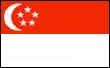
\includegraphics[width=5cm]{articles/Fiche-de-singapour/1210328633arj0.jpg}
%Drapeau de Singapour.
\smallbreak


\textbf{\textsc{Situation}}

\textbf{Présentation générale}

A l'extrême sud est de la péninsule malaise, la République de Singapour occupe une position stratégique à l'entrée du détroit de Malacca, qui longe la Malaisie au nord et Sumatra au sud. Sa superficie de 682,7 km2 se répartit entre une île principale d'environ 42 km (est-ouest) sur 23 km (nord-sud) et une soixantaine d'îlots. Séparée de la Malaisie par le détroit de Johore, d'à peine un kilomètre de large, elle est reliée au continent par une digue routière et ferroviaire, le "Causeway", et un pont à Tuas. Au sud, le détroit de Singapour la sépare de l'archipel indonésien de Riau. Le point culminant de l'île, le Timah Peak, est à 165 mètres au dessus du niveau de la mer.

\textbf{Liaisons avec la France}

11.000 km séparent Singapour de la France. Air France, Singapore Airlines et Quantas assurent des liaisons aériennes directes quotidiennes. Il existe par ailleurs de nombreux vols avec escales via Kuala Lumpur, Bangkok ou plusieurs capitales ou villes européennes (Londres, Amsterdam, Copenhague, Francfort...). Un vol direct dure environ 12h30.

\textbf{\textsc{Population}}

Principalement concentrée dans le sud de l'île, la population de 4 millions d'habitants compte 2,5 millions de Chinois, 382.000 Malais, 258.000 Indiens. Entre 1990 et 2000, la population non-résidente (étrangers vivant à Singapour depuis au moins un an) a presque doublé, passant de 10 à 19\% tandis que la part des résidents permanents s'élève à 7,2\%. En juin 2001, la population active comptait 2,12 millions de personnes.

|                                       |     SINGAPOUR   |    FRANCE    |
| ------------------------------------- |: -------------: | -----------: |
|Population                             |       4 millions| 59,2 millions|
|Densité                                |     6.055 hab.km2|   108 hab.km2|
|Accroissement naturel de la population |              1,7|           0,4|
|Indice de fécondité                    |              1,4|           1,8|
|Espérance de vie                       |           78 ans|      78,5 ans|
|Urbanisation                           |            100 \%|        75,6 \%|

\textbf{\textsc{Climat}}

Le climat est de type équatorial, chaud et humide toute l'année, avec une saison de fortes pluies de novembre à février. Les violents orages se montrent fréquents. La moyenne annuelle des températures s'établit de 24 à 34 degrés. Il n'y a pratiquement pas de variations saisonnières ni d'écart thermique entre le jour et la nuit. La pluviométrie annuelle moyenne est de 2500 mm. L'hygrométrie moyenne est de 84\%, avec un maximum de 96\% et un minimum de 64\%.

\textbf{\textsc{Villes principales}}

\textbf{Singapour}
Dans une mosaïque cosmopolite de quartiers (Chinatown, Kampong Glam, Little India, Orchard Road...), le centre ville, qui concentre les édifices publics et les hautes tours des affaires, se situe au sud de l'île. Entièrement reconstruit suivant un plan très aéré, il est doté de nombreux espaces verts. Des villes nouvelles entièrement constituées de blocs construits par le "Housing Development Board" se sont créées dans les banlieues : Ang Mo Kio, Bedok, Tampines, Clementi, Jurong. L'aéroport international de Changi, l'un des plus performants au monde, se trouve à l'est, sur l'île principale.

\end{multicols}

\vfill
